\documentclass[border=2pt]{standalone}

\usepackage{tikz}
\tikzset{>=latex}

\begin{document}
	
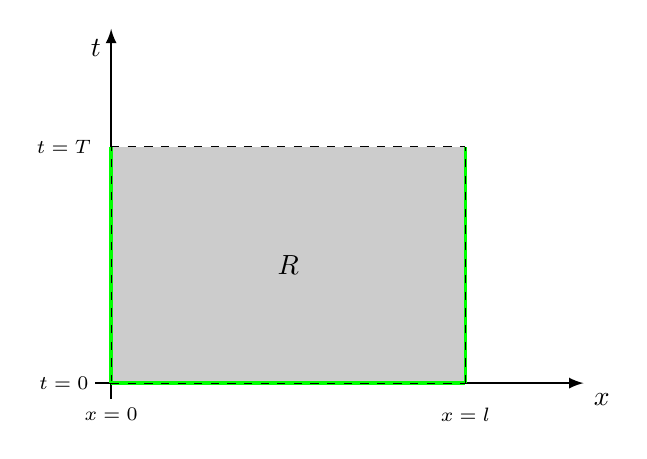
\begin{tikzpicture}
	%\draw[help lines] (0,0) grid (5,5);
	\path[fill=black!20] (0,0) -- (4.5,0) -- (4.5,3) -- (0,3);
	\draw[thick, ->] (-0.2,0) -- (6,0) node [below right] {$x$};
	\node at (0,-0.4) {\scriptsize$x=0$};
	\node at (4.5,-0.4) {\scriptsize$x=l$};
	\draw[thick, ->] (0,-0.2) -- (0,4.5) node [below left] {$t$};
	\node at (-0.6,0) {\scriptsize$t=0$};
	\node at (-0.6,3) {\scriptsize$t=T$};
	\draw[green, very thick] (4.5,0) -- (4.5,3);
	\draw[dashed] (4.5,0) -- (4.5,3);
	\draw[green, very thick] (0,0) -- (0,3);
	\draw[dashed] (0,0) -- (0,3);
	\draw[green, very thick] (0,0) -- (4.5,0);
	\draw[dashed] (0,0) -- (4.5,0);
	\draw[dashed] (0,3) -- (4.5,3);
	\node at (2.25,1.5) {$R$};
\end{tikzpicture}
	
\end{document}